\section{Approximations as Tangents}
\label{sec:approx-as-tangents}

We motivate our approach to \GPS by showing how to combine ideas from differential geometry and stable domain theory to reconstruct \GPS in a denotational setting. From this basis, we apply the CHAD framework of V{\'a}k{\'a}r \etal to obtain a denotational model of automatic differentiation that gives us an effective way to interpret programs as functions along with their forward and backwards approximation maps\bob{and we did it in Agda, so we can run it}.

\subsection{Manifolds, Smooth Functions, and Automatic Differentiation}

% For what follows we do not need to know in detail what a manifold is, or exactly how smooth functions are defined. We only state some definitions in order to fix terminology and to justify our claim of a connection to manifolds and smooth functions. \bob{Need a good reference here.}

The general study of differentiable functions takes place on \emph{manifolds}, which are topological spaces that ``locally'' look like a subset of the Euclidean space $\RR^n$. The spaces $\RR^n$ themselves are manifolds, but so are ``non-flat'' examples such as $n$-spheres and yet more exotic spaces. Every point $x$ in a manifold $M$ has an associated \emph{tangent vector space} $\tangents_x(M)$ and \emph{cotangent vector space} $\cotangents_x(M)$, the latter consisting of linear functions $\tangents_x(M) \linearto \RR$. The tangent and cotangent spaces are finite dimensional, so in the presence of a chosen basis they are canonically isomorphic. In the case when the manifold is $\RR^n$, then every tangent space is isomorphic to $\RR^n$ as well.

Smooth functions $f$ between manifolds $M$ and $N$ are functions on their points that are locally differentiable on $\RR^n$. Manifolds and smooth functions form a category $\Man$. Each smooth function induces maps of the (co)tangent spaces:
\begin{itemize}
\item The \emph{forward derivative} (tangent map or pushforward) $\pushf{f}_x$ is a linear map $\tangents_x(M) \linearto \tangents_{f(x)}(N)$. In the Euclidean case when $M = \RR^m$ and $N = \RR^n$, the tangent map can be represented by the Jacobian matrix of partial derivatives of $f$ at $x$.
\item The \emph{backward derivative} (cotangent map, or pullback) $\pullf{f}_x$ is a linear map $\cotangents_{f(x)}(N) \linearto \cotangents_x(M)$. In the Euclidean case, the backward derivative is represented by the transpose of the Jacobian of $f$ at $x$.
\end{itemize}

Computing the forward and backward derivatives of smooth functions $f$ has many applications of practical interest. For example, computation of the reverse derivative is of central interest in machine learning by gradient descent, the main technique used to train deep neural networks~\cite{rumelhart88,goodfellow16}.

Derivatives can be computed numerically by computing $f$ on small perturbations of its input, or symbolically by examining a closed-form representation of $f$. However, a more common and practical technique is to use \emph{automatic differentiation}, where a program computing $f$ is instrumented to produce (a representation of) the forward and/or backward derivative as a side-effect of producing the output. \bob{cite something on autodiff}. This has led to the area of differentiable programming, where programming languages and their implementations are specifically designed to admit efficient automatic differentation algorithms~\cite{jax2018github}. \bob{cite: TensorFlow, Dex, Jesse Sigal, etc.}

\subsection{Stable Domain Theory as Differentiability}

Our thesis is that \GPS is a form of differentiable programming, where tangents are not linear approximations of functions but instead are qualitiative approximations of elements in the sense of domain theory. Smooth functions in this setting are Berry's \emph{stable functions} \cite{berry79,berry82}. We now introduce these concepts and how they relate to \GPS.

\subsubsection{Domains as a Qualitative Theory of Approximation}

Domain theory is a method for defining the semantics of programs that handle infinite data (e.g., functions or infinite streams). \emph{Domains} are certain partially ordered sets where the ordering denotes a relationship of qualitative information content: if $x \sqsubseteq y$, then $y$ may contain more information than $x$. For example, if $x$ and $y$ are functions, then $y$ may be defined for more values in its domain than $x$. Infinite objects are understood in terms of their approximations in this sense, and domains are assumed to be closed under least upper bounds (lubs) of directed sets, meaning that any internally consistent collection of elements has a ``completion'' that contains all the information covered by the set. Programs are interpreted as monotone functions that preserve directed lubs. Monotonicity captures the idea that if the input gets more defined, then the output can get more defined. Preservation of lubs, or \emph{continuity}, states that a function interpreting a program cannot act inconsistently on approximations and their completion, which corresponds to the intuitive idea that a function that is computable cannot look at a non-finite amount of input to produce a finite output.

For the purposes of \GPS, we are not interested in using approximations to model computation on infinite objects, but instead to use them for the related use of revealing how programs explore their inputs when producing parts of their output. Therefore, we ignore completeness properties of the partially ordered sets we consider.

\subsubsection{Bounded Meets and Conditional Multiplicativity}
\label{sec:bounded-meets-and-cm}

When giving a denotational semantics for sequential programming languages, such as PCF, continuous functions are too permissive. Plotkin's Parallel OR (\exref{parallel-or}, below) is continuous but does not explore its input in a way consistent with a sequential implementation \cite{plotkin77lcf}. Continuous functions can explore their input in a ``random access'' way, which is incompatible with the central idea in \GPS that we should be able to identify a \emph{minimal} part of the input that leads to a part of the output.

Stability is a property that can be required of monotone functions that was invented by \citet{berry79} in an attempt to capture sequentiality. This was not successful (see the $\mathrm{gustave}$ function in \exref{parallel-or}), but we will see now how it is closely related to problem of computing forward and backwards maps of approximations needed in \GPS. A textbook description of stable functions in the context of domain theory is given by \citet{amadio-curien} (Chapter 12). We start with a property that is weaker than stability, but is easier to motivate in connection with derivatives of smooth functions.

In a partially ordered set $X$, for any $x \in X$ the set of elements below $x$, $\downset{x} = \{ x' \mid x' \sqsubseteq x \}$, is itself a partially ordered set. These approximations of $x$ we will think of as ``derivatives'' of $x$, and the whole set $\downset{x}$ as the ``tangent space''. Tangent spaces are vector spaces, since they are linear approximations to curves at that point. In the partially ordered setting, we take elements of $\downset{x}$ to be approximations of processes defined at $x$. As we can add tangents, we assume we can take meets of approximations in $\downset{x}$:

\begin{definition}
  A \emph{bounded meet poset} is a partially ordered set $X$ where for every $x \in X$, $\downset{x}$ is a meet semilattice, with $x$ as the top element.
\end{definition}

Smooth functions have a ``pushforward'' derivative that takes tangents at a point $x$ to tangents at the point $f(x)$ and is linear. In the partially ordered setting, we are going to take a function $f$'s pushforward derivative at $x$ to be its restriction to $\downset{x}$, taking approximations of the input to approximations of the output. Matching the linearity of the pushforward derivative smooth functions, we require that these restrictions preserve meets:

\begin{definition}
  A \emph{conditionally multiplicative} (cm) function $f : X \to Y$ is
  a monotone function such that for all $x \in X$, the restriction
  $f_x : \downset{x} \to \downset{f(x)}$ preserves meets.
\end{definition}

\begin{lemma}
  Morphisms of meet approximation spaces are closed under identities
  and composition, forming a category. FIXME: with products?
  functions? sums?
\end{lemma}

\begin{example}[Conditionally Multiplicative Functions]
\label{ex:strict-short-circuit}
  To see the effect of requiring preservation of bounded meets,
  consider several ways of defining disjunction on the lifted booleans
  $\mathbb{B}_\bot$. Two functions that are cm are the strict and
  left-short-circuiting ORs\footnote{The clauses in these examples are
    shorthand for the graph of the function. They are not to be
    understood as pattern matching clauses in a language like Haskell,
    where it is not possible to match on $\bot$.}:
  \begin{displaymath}
    \begin{array}[t]{l@{(}l@{,~}l@{)~}c@{~}l}
      \mathrm{strictOr}&\mathsf{tt}&\mathsf{tt}&=&\mathsf{tt} \\
      \mathrm{strictOr}&\mathsf{tt}&\mathsf{ff}&=&\mathsf{tt} \\
      \mathrm{strictOr}&\mathsf{ff}&\mathsf{tt}&=&\mathsf{tt} \\
      \mathrm{strictOr}&\mathsf{ff}&\mathsf{ff}&=&\mathsf{ff} \\
      \mathrm{strictOr}&\bot&\_&=&\bot \\
      \mathrm{strictOr}&\_&\bot&=&\bot \\
    \end{array}
    \qquad
    \begin{array}[t]{l@{(}l@{,~}l@{)~}c@{~}l}
      \mathrm{shortCircuitOR}&\mathsf{tt}&\_&=&\mathsf{tt} \\
      \mathsf{shortCircuitOR}&\mathsf{ff}&x&=&x \\
      \mathsf{shortCircuitOR}&\bot&\_& =& \bot
    \end{array}
    \qquad
    \raisebox{-15ex}{
      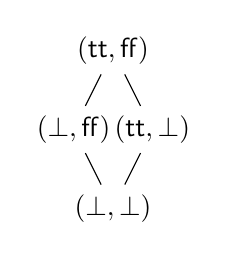
\begin{tikzpicture}
        \node (top) at (0,0) {$(\mathsf{tt},\mathsf{ff})$};
        \node [below of=top,xshift=-0.5cm] (oi) {$(\bot,\mathsf{ff})$};
        \node [below of=top,xshift=0.5cm] (io) {$(\mathsf{tt},\bot)$};
        \node [below of=oi,xshift=0.5cm] (oo) {$(\bot,\bot)$};
        \draw (top) -- (oi);
        \draw (top) -- (io);
        \draw (oi) -- (oo);
        \draw (io) -- (oo);
      \end{tikzpicture}
    }
  \end{displaymath}
  In the poset $\mathbb{B}_\bot^2$, a typical poset of approximations of a fully defined element is shown to the right. For $\mathrm{strictOr}$, any approximation that isn't the fully defined input is mapped to $\bot$, while $\mathrm{shortCircuitOr}$ maps the partially defined $(\mathsf{tt},\bot)$ to $\mathsf{tt}$. Thus, even though these functions operate identically on fully defined inputs, they differ in their \emph{derivatives} on partially defined input, exposing how . That they are cm can be checked by examining their restrictions' behaviour. If we take the approximations $(\bot,\mathsf{ff})$ and $(\mathsf{tt},\bot)$, then their meet is $(\bot,\bot)$; $\mathrm{strictOr}$ maps all three elements to $\bot$, so is cm here since $\bot \wedge \bot = \bot$; and $\mathrm{shortCircuitOR}$ has $(\bot,\mathsf{ff}) \mapsto \bot$ and $(\mathsf{tt},\bot) \mapsto \mathsf{tt}$, the meet of which is $\bot = \mathrm{shortCircuitOR}(\bot,\bot)$. Other combinations can be checked similarly.
\end{example}

\begin{example}[A non-Conditionally Multiplicative Function]
  \label{ex:parallel-or}
  A function that is not cm is Plotkin's Parallel OR \cite{lcf77}, which short-circuits in both arguments. It returns $\mathsf{tt}$ if either argment is $\mathsf{tt}$ even if the other argument is not defined:
  \begin{displaymath}
    \begin{array}{l@{(}l@{,~}l@{)~}c@{~}l}
      \mathrm{parallelOR}&\mathsf{tt}&\_&=&\mathsf{tt} \\
      \mathrm{parallelOR}&\_&\mathsf{tt}&=&\mathsf{tt} \\
      \mathsf{parallelOR}&\mathsf{ff}&\mathsf{ff}&=&\mathsf{ff} \\
      \mathsf{parallelOR}&\bot&\bot&=&\bot
    \end{array}
  \end{displaymath}
  We have $\mathrm{parallelOR}(\mathsf{tt}, \bot) \wedge \mathrm{parallelOR}(\bot, \mathsf{tt}) = \mathsf{tt} \wedge \mathsf{tt} = \mathsf{tt}$ but $\mathrm{parallelOR}((\mathsf{tt},\bot) \wedge (\bot, \mathsf{tt})) = \mathrm{parallelOR}(\bot, \bot) = \bot$, so it is not cm.

  Parallel OR is famous because it is not \emph{sequential}, meaning intuitively that it cannot be implemented without running the two arguments in parallel to see if one of them returns $\mathsf{tt}$. The fact that it exists in the standard domain theoretic semantics of PCF means that this semantics is incomplete for reasoning about observational equivalence in PCF. Since Parallel OR is not cm, one might hope that cm-ness is enough to capture sequentiality, and hence potentially give a fully abstract model of PCF. However, the following ternary function $\mathbb{B}_\bot^3 \to \{\top,\bot\}$ is cm but admits no sequential implementation that fixes an order that the arguments are examined in:
  \begin{displaymath}
    \begin{array}{l@{(}l@{,~}l@{,~}l@{)~}c@{~}l}
      \mathrm{gustave}&\mathsf{tt}&\mathsf{ff}&\_&=&\top \\
      \mathrm{gustave}&\mathsf{ff}&\_&\mathsf{tt}&=&\top \\
      \mathrm{gustave}&\_&\mathsf{tt}&\mathsf{ff}&=&\top \\
      \mathrm{gustave}&\_&\_&\_&=&\bot
    \end{array}
  \end{displaymath}
  Due to the way that the cases are defined, there is no way of constructing a pair of approximations for which preservation of their meet does not hold. In terms of derivatives, this makes sense in that we are only concerned about the intensional behaviour of a function at a point and its approximations. Parallel OR has two incompatible approximation behaviours at the point $(\mathsf{tt},\mathsf{tt})$. The $\mathrm{gustave}$ function does have consistent behaviour at each approximation for each point.
\end{example}

Conditional multiplicativity seems to be a reasonable analogue to functions with a well-defined notion of derivative. However, for \GPS we also require an analogue to the reverse derivative, where we map approximations backwards to give the least approximation of the input for a given approximation of the output. In the case of smooth functions, we are always guaranteed a reverse derivative but there is not always a best way to map approximations backwards for cm functions, as the following example shows.

\begin{example}[Is Conditional Multiplicativity Enough?]
  \label{ex:non-stable-function}
  % In the preceeding examples, we demonstrated conditional
  % multiplicativity by giving a backwards mapping of approximations
  % that forces preservation of meets. A natural question is whether or
  % not we always have such a backwards map which we could use for
  % backwards propagation of approximations.
  An example that is conditionally multiplicative, but does not admit a backards map of approximations (from \citet{amadio-curien} just before Lemma 12.2.3, originally due to Berry) is given by defining $\mathrm{unstable} : D \to \{\bot, \top\}$, where:
  \begin{displaymath}
    D = \bot \sqsubseteq \cdots \sqsubseteq n \sqsubseteq \cdots \sqsubseteq 1 \sqsubseteq 0
  \end{displaymath}
  as $\mathrm{unstable}(\bot) = \bot$ and $\mathrm{unstable}(n) = \top$. This is monotone, and preserves meets in every $\downset{x}$. However, there is no ``best'' (i.e., least) input that gives us any finite output.
\end{example}

\subsubsection{Stable functions and L-posets}

In light of the preceeding example, we can give an alternative
definition of a function that requires the existence of a reverse
mapping directly, even without assuming that any meets exist:

\begin{definition}[Stable function]
  Let $f : X \to Y$ be a monotone function between posets $X$ and
  $Y$. The function $f$ is \emph{stable} if for all $x \in X$ and
  $y \leq f(x)$:
  \begin{enumerate}
  \item (\textsc{Existence}) there exists an $x_0 \leq x$ such that $y \leq f(x_0)$, and
  \item (\textsc{Minimality}) for any $x'_0 \leq x$ such that $y \leq f(x'_0)$ then
    $x_0 \leq x'_0$ .
  \end{enumerate}
\end{definition}

\begin{example}
  \begin{enumerate}
  \item The function $\mathrm{strictOr}$ is stable. For example, for the input-output pair $(\mathsf{tt},\mathsf{ff}) \mapsto \mathsf{tt}$, the minimal input that gives this output is exactly $(\mathsf{tt}, \mathsf{ff})$. If we take the approximation $\bot \leq \mathsf{tt}$ of the output, then the corresponding minimal input is $(\bot, \bot)$. The function $\mathrm{shortCircuitOR}$ is also stable. For the input-output pair $(\mathsf{tt},\mathsf{ff}) \mapsto \mathsf{tt}$, the minimal input that gives this input is $(\mathsf{tt},\bot)$, indicating that the presence of $\mathsf{ff}$ in the second argument was not necessary to produce this output. As with $\mathrm{strictOr}$, the minimal input required to produce the output $\bot \leq \mathsf{tt}$ is again $(\bot,\bot)$.

  \item The $\mathrm{parallelOR}$ function is not stable. For the input-output pair $(\mathsf{tt},\mathsf{tt}) \mapsto \mathsf{tt}$, there is no one minimal input that produces this output. We have both $\mathrm{parallelOR}(\mathsf{tt},\bot) = \mathsf{tt}$ and $\mathrm{parallelOR}(\bot,\mathsf{tt}) = \mathsf{tt}$, which are incomparable and their greatest lower bound $(\bot,\bot)$ gives the output $\bot$.

  \item The $\mathrm{gustave}$ function is stable. Despite there being no one minimal input that achieves the output $\top$, each of the minimal inputs that can achieve this output are pairwise incomparable, so for each specific input that gets output $\top$ there is a unique minimal input that achieves it (listed in the first three lines of the definition).

    In terms of \GPS the $\mathrm{gustave}$ function does not present a problem. For any particular run (i.e., input$\mapsto$output pair), there is an unambiguous minimal input that achieves the output, no matter that it was not achieved by a sequential processing of the input.

  \item As discussed above, $\mathrm{unstable}$ is not stable, but is conditionally multiplicative.
  \end{enumerate}
\end{example}

The fact that these two functions's stability witnesses reveal information about how they depend on their input is what we will exploit in order to use the idea of stability for \GPS. It is interesting that sequentiality is not necessarily required in order to obtain backwards maps of approximations, as might be assumed by thinking about how to trace computations for provenance information.

Stability has an alternative definition in terms of Galois connections, which will be more useful for what follows. This characterisation is due to Paul Taylor\bob{cite}. We first formally define Galois connections, which we used informally in \exref{introduction-example}.

\begin{definition}[Galois connection]
  \label{def:galois-connection}
  Suppose $X$ and $Y$ are posets. A \emph{Galois connection} $f \adj g: X \to Y$ is a pair of monotone functions $f: Y \to X$ and $g: X \to Y$ satisfying $y \leq g(x) \iff f(y) \leq x$ for any $x \in X$ and $y \in Y$. We refer to $f$ as the left adjoint and $g$ as the right adjoint.
\end{definition}

\begin{lemma}
  A monotone function $f : X \to Y$ is stable if and only if for all $x \in X$, the restriction of $f_x : \downset{x} \to \downset{f(x)}$ has a left Galois adjoint.
\end{lemma}

\begin{proof}
  If $f$ is stable, then define a left adjoint
  $f^*_x : \downset{f(x)} \to \downset{x}$ by setting $f^*_x(y)$ to be
  the minimal $x_0$ required by stability. This is monotone: if
  $y \leq y'$, then we know that $y \leq y' \leq f(f^*_x(y'))$ by
  definition of $f^*_x$, so $f^*_x(y) \leq f^*_x(y')$ by minimality of
  $f^*_x(y)$. For the adjointness, let $x' \leq x$ and $y \leq
  f(x)$. Then if $f^*_x(y) \leq x'$, we have
  $y \leq f(f^*_x(y)) \leq f(x')$ by monotonicity of $f$ and the first
  part of stability. In the other direction, if we have
  $y \leq f(x')$, then by uniqueness we have $f^*_x(y) \leq x'$.

  If, for every $x$, $f_x$ has a left adjoint $f^*_x$, then for any
  $x', y$ we have $y \leq f_x(x') \Leftrightarrow f^*_x(y) \leq
  x'$. So $f^*_x(y)$ is the element that satisfies
  $y \leq f(f^*_x(y))$, and it is minimal since if $y \leq f_x(x'_0)$
  then $f^*_x(y) \leq x'_0$.
\end{proof}

Even though stable functions can be defined on any partially ordered set, in light of the analogy with tangent spaces, it makes sense to require that meets, preserved by forward approximation maps, and joins, preserved by backwards approximation maps, exist:

\begin{definition}
  An \emph{L-poset} is a partially ordered set $X$ such that for every $x \in X$, the principal downset $\downset{x}$ is a bounded lattice (i.e., have all finite meets and joins).
\end{definition}

This lemma is an instance of standard facts about Galois connections
preserving meets and joins:

\begin{lemma}
  For L-posets $X$ and $Y$, a stable function $f : X \to Y$ preserves
  meets in its forward part $f_x$ and joins in its reverse part
  $f^*_x$.
\end{lemma}

The converse to this lemma (that functions that preserve meets in their forward part have a left Galois adjoint) is not true, as was demonstrated by the non-stable function in \exref{non-stable-function}. In the case when the posets $\downset{x}$ are \emph{complete}, and $f_x$ preserves infinitary meets, then we are guaranteed a left Galois adjoint. In that example, the infinite set $\{0, 1, 2, \dots, n, n-1, \dots\}$ not including $\bot$ of approximations of $0$ does not have a greatest lower bound, so the order is not complete.

We could have required that L-posets' principal downsets were complete lattices, which would mean that we would only need to require that forward approximation maps preserve all meets and we could compute the backwards map automatically. However, our goal is a computable theory for \GPS, analogous to automatic differentiation. Requiring completeness to compute backwards maps of approximations would require that complete joins are always computable, which will not be the case for approximations of functions.

\begin{proposition}
  L-posets and stable functions form a category. \bob{and the main point is that composition of stability witnesses looks like a chain rule!}
\end{proposition}

\bob{L-poset is has products and coproducts, but is not closed. To be closed would require each $\downset{x}$ to be a \emph{complete} lattice. However, this is tricky to implement as we need an infinitary operation to compute the reverse approximation map for function types. See \cite{amadio-curien} for the proof that bounded-complete lattices with stable functions form a cartesian closed category.}

\subsection{Summary}
\label{sec:diff-stab-summary}

Let us summarise our analogy between differentiable functions between manifolds and stable functions between L-posets:

\begin{itemize}
\item For \GPS, we assume that every value has an associated lattice of {\em approximations}. For differentiable programs, every point has an associated vector space of {\em tangents}.
\item For \GPS, every program has an associated forward approximation map that takes approximations forward from the input to the output. This map {\em preserves meets}. For differentiable programs, every program has a forward derivative that takes tangents of the input to tangents of the output. The forward derivative map is {\em linear}, so it preserves addition of tangents and the zero tangent.
\item For \GPS, every program has an associated backward approximation map that takes approximations of the output back to least approximations of the input. This map {\em preserves joins}. For differentiable programs, every program has a reverse derivative that takes tangents of the output to tangents of the input. This map is again {\em linear}.
\item For \GPS, the forward and backward approximation maps are related by being a Galois connection. For differentiable programming, the forward and reverse derivatives are related by being each others' transpose.
\end{itemize}

\bob{Put a conjecture about Tangent Categories in somewhere}

Given this close connection between \GPS and differentiable programming, we can take structures intended for modelling automatic differentiation and use them to model \GPS. This will enable us to generalise and expand the scope of \GPS to act as a foundation for data provenance in a wide range of computational settings.
